\section{ HÀM SỐ BẬC HAI}
\subsection{TÓM TẮT LÝ THUYẾT}

\subsubsection{Hàm số bậc hai $y=ax^2+bx+c$, với $a \ne 0$.}
\begin{itemize}
	\item[\ding{172}] Tập xác định $\mathbb{R}$.
	\item [\ding{173}] Tọa độ đỉnh $S\left(-\dfrac{b}{2a};-\dfrac{\Delta}{4a} \right)$. \textit{Để xác định nhanh tọa độ đỉnh, ta chỉ cần xác định hoành độ $x_0$. Sau đó thay $x_0$ vào hàm số, ta tính $y_0$}.
	\item [\ding{174}] Sự biến thiên của hàm số bậc hai:\\
	\begin{minipage}[b]{7cm}
		\begin{khung4}{$a>0$}
			
\begin{tikzpicture}
				\tkzTabInit[lgt=1,espcl=2]
				{$x$/1,$y$/2}
				{$-\infty$,$-\dfrac{b}{2a}$,$+\infty$}
				\tkzTabVar{+/$+\infty$,-/$-\dfrac{\Delta}{4a}$,+/$+\infty$}
			\end{tikzpicture}
			\begin{itemize}
				\item $a>0$ thì bề lõm quay lên.
				\item Hàm số nghịch biến trên $\left(-\infty;-\frac{b}{2a} \right)$; đồng biến trên $\left(-\frac{b}{2a};+\infty \right)$.
			\end{itemize}
		\end{khung4}
	\end{minipage}\hspace{1cm}
	\begin{minipage}[b]{7cm}
		\begin{khung4}{$a<0$}
			
\begin{tikzpicture}
				\tkzTabInit[lgt=1,espcl=2]
				{$x$/1,$y$/2}
				{$-\infty$,$-\dfrac{b}{2a}$,$+\infty$}
				\tkzTabVar{-/$-\infty$,+/$-\dfrac{\Delta}{4a}$,-/$-\infty$}
			\end{tikzpicture}
			\begin{itemize}
				\item $a<0$ thì bề lõm quay xuống.
				\item Hàm số đồng biến trên $\left(-\infty;-\frac{b}{2a} \right)$; nghịch biến trên $\left(-\frac{b}{2a};+\infty \right)$.
			\end{itemize}
		\end{khung4}
	\end{minipage}
\end{itemize}

\subsubsection{Đồ thị hàm số bậc hai $y=ax^2+bx+c$, với $a \ne 0$.}

\begin{itemize}
	\item [\ding{172}] Trong mặt phẳng $Oxy$, đồ thị là một parabol:\\
	\hspace*{1cm}
	\begin{tikzpicture}[smooth,samples=300,scale=0.6,>=stealth]
		\draw[->] (-0.8,0)--(4.5,0) node[below]{$x$};
		\draw[->] (0,-1.5)--(0,2.5) node[right]{$y$};
		\draw (0,0) node[above left]{$O$};
		\draw[thick, magenta,domain=0.3:3.7] plot(\x,{(\x)^2-4*(\x)+3});
		\draw[fill=blue] (2,-1) circle(1.5pt) (2,0) circle(1pt) (0,-1) circle(1pt);
		\draw[dashed] (2,-1.5)--(2,2.5) (2,-1)--(0,-1)node[left]{\footnotesize$-\dfrac{\Delta}{4a}$};
		\node[right] at (2,2.4) {\footnotesize $x=-\tfrac{b}{2a}$};
		\node[right] at (0.5,-2) {\fbox{\footnotesize$a>0$}};
	\end{tikzpicture}
	\hspace*{4cm}
	\begin{tikzpicture}[smooth,samples=300,scale=0.6,>=stealth]
		\draw[->] (-0.8,0)--(4.5,0) node[below]{$x$};
		\draw[->] (0,-1.5)--(0,2.5) node[right]{$y$};
		\draw (0,0) node[above left]{$O$};
		\draw[thick, magenta,domain=0.2:3.8] plot(\x,{-(\x)^2+4*(\x)-2});
		\draw[fill=blue] (2,2) circle(1.5pt) (2,0) circle(1pt) (0,2) circle(1pt);
		\draw[dashed] (2,-1.4)--(2,2.5) (2,2)--(0,2)node[left]{\footnotesize$-\dfrac{\Delta}{4a}$};
		\node[right] at (2,-1.5) {\footnotesize $x=-\tfrac{b}{2a}$};
		\node[right] at (0.5,-2) {\fbox{\footnotesize$a<0$}};
	\end{tikzpicture}
	\item [\ding{173}] Trục đối xứng: $x=-\dfrac{b}{2a}$ (\textit{xem đồ thị}).
	\item [\ding{174}] Cắt trục tung tại điểm có tung độ bằng $c$, tức là đồ thị luôn qua điểm $(0;c)$.
	\item [\ding{175}] Giá trị lớn nhất (max), giá trị nhỏ nhất (min)
	\begin{itemize}
		\item Khi $a>0$, hàm số đạt \textbf{giá trị nhỏ nhất} $y_{\min} =-\dfrac{\Delta}{4a}$ khi $x=-\dfrac{b}{2a}$ (tại đỉnh).
		\item Khi $a<0$, hàm số đạt \textbf{giá trị lớn nhất} $y_{\max} =-\dfrac{\Delta}{4a}$ khi $x=-\dfrac{b}{2a}$ (tại đỉnh).
	\end{itemize}
\end{itemize}

\subsection{RÈN LUYỆN KĨ NĂNG GIẢI TOÁN}
\begin{dang}{Đồ thị hàm số bậc hai và các vấn đề liên quan}
	\indamm{Muốn vẽ parabol, ta cần là các bước sau:}
	\begin{listEX}[1]
		\item [\ding{172}] Xác định tọa độ đỉnh $S(x_0;y_0)$, với $x_0=-\dfrac{b}{2a}$, $y_0$ được tính bằng cách thay $x_0$ vào hàm số và bấm máy.
		\item [\ding{173}] Xác định trục đối xứng $d \colon x=-\dfrac{b}{2a}$.
		\item [\ding{174}] Lập bảng giá trị (5 điểm), hoặc tìm giao điểm với $Ox$, $Oy$.
		\item [\ding{175}] Xác định "chiều quay" của parabol và vẽ \indamm{parabol} có đỉnh $S$, có trục đối xứng $d$ và qua các điểm vừa xác định. 
	\end{listEX}
\end{dang}

\begin{vd}%[0D2Y3]
	Cho hàm số $y=-x^2-3x+1$ có đồ thị là parabol $(P)$. 
	\begin{tasks}(1)
		\task Tìm tọa độ của đỉnh, giao điểm của đồ thị $(P)$ với trục tung và trục hoành.
		\task Tìm các khoảng đồng biến và nghịch biến của hàm số.
	\end{tasks}
\end{vd}\dongcham{10}
\begin{vd}%[0D2Y3]
	Cho hàm số $y=x^2-4x+3$ có đồ thị là parabol $(P)$. 
	\begin{tasks}
		\task Tìm các khoảng đồng biến và nghịch biến của hàm số. 
		\task Vẽ đồ thị $(P)$.
	\end{tasks}
\end{vd}\dongcham{10}

\begin{vd}
	Vẽ đồ thị và xác định tập giá trị của các hàm số sau đây
	\begin{listEX}[3]
		\item $y=2x^2$.
		\item $y=x^2-4x+1$.
		\item $y=-x^2-2x+3$.
		\item $y=-x^2-2$.
		\item $y=-\dfrac{1}{4}x^2+\dfrac{3}{2}x+\dfrac{7}{4}$.
		\item $y=\dfrac{2}{3}x^2-\dfrac{4}{3}x+2$.
	\end{listEX}
\end{vd}\dongcham{36}

\begin{dang}{Xác định hàm số bậc hai $y=ax^2+bx+c$}
	Việc xác định $(P)$ hay đi tìm các hệ số $a$, $b$, $c$, ta thường quy về việc giải hệ phương trình liên quan đến ba ẩn  $a$, $b$, $c$. Khi tìm các phương trình liên quan, ta chú ý một số nội dung sau:
	\begin{itemize}
		\item[\iconMT] Nếu đề cho $(P)$ qua điểm $(x_0;y_0)$ thì ta được: $ax_0^2+bx_0+c=0$.
		\item[\iconMT] Nếu đề cho tọa độ đỉnh là $(x_0;y_0)$ thì ta được
		\begin{listEX}[1]
			\item [\ding{172}] Hoành độ đỉnh $-\dfrac{b}{2a}=x_0$;
			\item [\ding{173}] $(x_0;y_0) \in (P)$, suy ra $ax_0^2+bx_0+c=0$.
			\item [\ding{174}] $(P)$ viết dưới dạng $y=a(x-x_0)^2+y_0$.
		\end{listEX}
		\item[\iconMT] Nếu đề cho hoành độ đỉnh (hoặc trục đối xứng) $x=x_0$, ta được $-\dfrac{b}{2a}=x_0$.
		\item[\iconMT] Nếu đề cho tung độ đỉnh $y=y_0$, ta được $-\dfrac{\Delta}{4a}=y_0$.
	\end{itemize}
\end{dang}
\begin{vd}
	Xác định phương trình của $(P)\colon y=-2x^2+bx+c$, biết
	\begin{tasks}
		\task $(P)$ đi qua hai điểm $M(0;-2)$ và $N(2;0)$;
		\task $(P)$ có đỉnh $I(1;3)$;
		\task $(P)$ đi qua điểm $A(2;-3)$ và có hoành độ đỉnh $x_0=3$;
		\task $(P)$ có trục đối xứng là $x=2$ và cắt trục hoành tại điểm có hoành độ bằng $2$.
	\end{tasks}
\end{vd}\dongcham{19}

\begin{vd}
	Xác định hàm số $y=ax^2+bx+c$ có đồ thị $(P)$, biết 
	\begin{tasks}
		\task $(P)$ đi qua ba điểm $A(1;0)$, $B(2;8)$ và $C(0;-6)$.
		\task $(P)$ đi qua điểm $A(0;5)$ và có đỉnh $I(3;-4)$.
		\task Hàm số đạt giá trị nhỏ nhất bằng $3$ và đồ thị $(P)$ qua các điểm $(0;5)$, $(3;13)$.
	\end{tasks}
\end{vd}\dongcham{14}

\begin{vd}
	Hãy viết phương trình của parabol ứng với mỗi đồ thị dưới đây.
	\begin{listEX}[2]
		\item \begin{tikzpicture}[smooth,samples=300,scale=0.5,>=stealth]
			\draw[->] (-7,0)--(2,0) node[above]{$x$};
			\draw[->] (0,-5)--(0,1.5) node[right]{$y$};
			\draw (0,0) node[above left]{$O$};
			\draw[domain=-6.3:0.35] plot(\x,{-4/9*(\x)^2-8/3*(\x)-4});
			\draw[fill=black] (-3,0) circle(1.5pt) (0,-4) circle(1.5pt);
			\draw[dashed] (-3,0)--(-3,-4.7);
			\node[above] at (-3,0) {\small $-3$};
			\node[right] at (0,-4) {\small $-4$};
		\end{tikzpicture}
		\item \begin{tikzpicture}[smooth,samples=300,scale=0.8,>=stealth]
			\draw[->] (-4,0)--(2,0) node[below]{$x$};
			\draw[->] (0,-1.5)--(0,2) node[right]{$y$};
			\draw (0,0) node[above left]{$O$};
			\draw[domain=-3.5:1.5] plot(\x,{4/9*(\x)^2+8/9*(\x)-5/9});
			\draw[fill=black] (-1,-1) circle(1.5pt) (0.5,0) circle(1.5pt) (-1,0) circle(1pt) (0,-1) circle(1pt);
			\draw[dashed] (0,-1)--(-1,-1)--(-1,2);
			\node[left] at (0,-1.3) {\small $-1$};
			\node[above] at (-1.3,0) {\small $-1$};
			\node[below] at (0.7,0) {\small $\dfrac{1}{2}$};
		\end{tikzpicture}
	\end{listEX}
\end{vd}\dongcham{15}


\begin{dang}{Ứng dụng của hàm số bậc hai trong thực tế}
	\begin{itemize}
		\item [\iconMT] Một số mô hình thực tế (cổng chào, cầu,...) có hình dạng parabol;
		\item [\iconMT] Một số chuyển động có phương trình quỹ đạo là một hàm bậc hai.
	\end{itemize}
	Khi thực hiện đo đạc tính toán, ta thường dùng lý thuyết về hàm số bậc hai để giải các bài toán trên.
\end{dang}

\begin{vd}%[0D2T3]
	Một vật chuyển động với vận tốc $v=40+18t-t^2$ (m/s). Trong $20$ giây đầu vận tốc lớn nhất của vật là bao nhiêu?

	\loigiai{
		\immini{Đồ thị của hàm vận tốc $v$ có dạng Parabol  bề lõm hướng xuống dưới. Đỉnh của Parabol là $I(9;121)$. Do đó trong đoạn $[0;20]$, vận tốc lớn nhất của vật là $121$ m/s.
		}{
			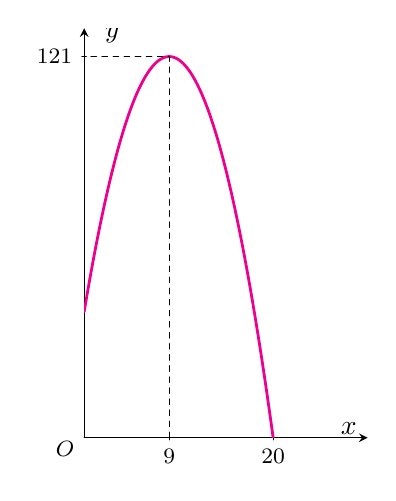
\begin{tikzpicture}[line cap=round,line join=round,>=stealth,x=0.3cm,y=0.1cm, scale=0.4]
				\draw[->,color=black] (0,0.) -- (30,0.);
				\foreach \x in {9,20}
				\draw[shift={(\x,0)},color=black] (0pt,2pt) -- (0pt,-2pt) node[below] {\footnotesize $\x$};
				\draw[->,color=black] (0.,0) -- (0.,130);
				\foreach \y in {121}
				\draw[shift={(0,\y)},color=black] (2pt,0pt) -- (-2pt,0pt) node[left] {\footnotesize $\y$};
				\draw[color=black] (0pt,-10pt) node[left] {\footnotesize $O$};
				\clip(0,0) rectangle (30,130);
				\draw[line width=1pt,color=magenta,smooth,samples=100,domain=0:20] plot(\x,{40+18*\x-(\x)^2});
				\draw [dash pattern=on 2pt off 2pt] (9,0)--(9,121)--(0,121);
				\draw (28, 3)  node {$x$}; \draw (3,128)  node {$y$};
			\end{tikzpicture}
	}}
\end{vd}\dongcham{14}

\begin{vd}%[0D2G3-5]%
	Một cuốn tạp chí bán giá $20$ ngàn đồng, chi phí xuất bản $x$ cuốn là
	\[ C(x)=0,0001x^2-0,2x+10.000 \,\, \, (\text{đơn vị 10.000 đồng})\]
	Chi phí phát hành mỗi cuốn là $4$ ngàn đồng; Các khoản thu bao gồm tiền bán tạp chí và $90$ triệu đồng tiền quảng cáo. Tìm số lượng tạp chí cần xuất bản để có mức lãi cao nhất? (\textit{Giả thiết số cuốn tạp chí in ra được bán hết})
	\loigiai
	{
		Ta có: Lãi = Tổng thu - tổng chi.\\
		+ Tổng thu $R(x) = 2x+\dfrac{90.10^6}{10^4}=2x+9000$.\\
		+ Tổng chi $T(x) = C(x)+0,4x =0,0001x^2+0,2x+10000$.\\
		Suy ra lãi $I(x) = R(x)-T(x)=-0,001x^2+1,8x-1000$. Khi đó biểu thức $I(x)$ là một parabol có đỉnh $I(9000;I(9000))$ và có bảng biến thiên
		\begin{center}
			
\begin{tikzpicture}
				\tkzTabInit[lgt=1.5,espcl=2.0,deltacl=.5,nocadre]
				{$x$ /0.7,$I(x)$ /1.7}
				{$0$ , $9000$ , $+\infty$}
				%\tkzTabLine{,-,0,+,0,-,}
				\tkzTabVar{-/$-1000$ ,+/$I(9000)$, -/$-\infty$}
			\end{tikzpicture}
		\end{center}
		Từ bảng biến thiên suy ra để lãi $I(x)$ cao nhất phải sản xuất $9000$ cuốn tạp chí.
	}
\end{vd}\dongcham{14}

\begin{vd}%[0D2T3]
	\immini{
		Một chiếc cổng hình Parabol bao gồm một cửa chính hình chữ nhật ở giữa và hai cánh cửa phụ hai bên như hình vẽ. Biết chiều cao cổng Parabol là $4$ m còn kích thước cửa ở giữa là $3$ m $\times$ $4$ m. Hãy tính khoảng cách giữa hai điểm $A$ và $B$. (xem hình minh họa bên).
		}
	{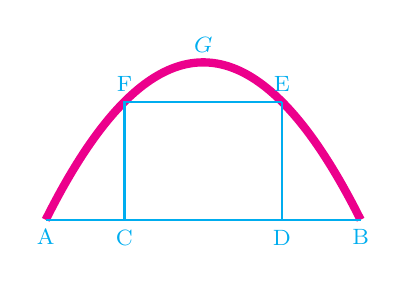
\begin{tikzpicture}[scale=0.5,thick,>=stealth,font=\footnotesize,cyan]
			\draw[line width=3pt,magenta,smooth,samples=100,domain=-4:4] plot(\x,{-0.25*(\x)^2});
			\draw[dashed,thin](2,-1)node[above]{ E};
			\draw[dashed,thin](-2,-1)node[above]{F};
			\draw[dashed,thin](-4,-4)node[below]{ A};
			\draw[dashed,thin](4,-4)node[below]{B};
			\draw[thick](2,-1)--(-2,-1)--(-2,-4)node[below]{ C}--(2,-4)node[below]{D}--(2,-1);
			\draw[thick](-4,-4)--(4,-4);
			\draw (0,0) node[above] { $G$};
		\end{tikzpicture}
	}
	\loigiai
	{\immini{Chọn hệ trục tọa độ $Oxy$ như hình vẽ với $O\equiv G$.\\Gọi phương trình của parabol là $y=ax^2+bx+c, a\neq 0$.\\Do parabol đi qua gốc tọa độ $O$ nên $c=0$.\\Do parabol có trục đối xứng $x=0$ nên $b=0\Rightarrow (P): y=ax^2$.\\Do kích thước cửa ở giữa là $3$ m $\times$ $4$ m và chiều cao cổng parabol là $4$ m nên $OI=4$ m, $HI=3$ m, $CD=4$ m $\Rightarrow HE=2$ m, $OH=1$ m $\Rightarrow E(2;-1)$ và $B\left(x_B; -4\right)$ với $x_B>0$.\\Do $E\in (P)$ nên tìm được $a=-\dfrac{1}{4}\Rightarrow (P): y=-\dfrac{1}{4}x^2$.\\Do $B\in (P)$ nên tìm được $x_B=4$. Vậy $AB=8$ m.}
		{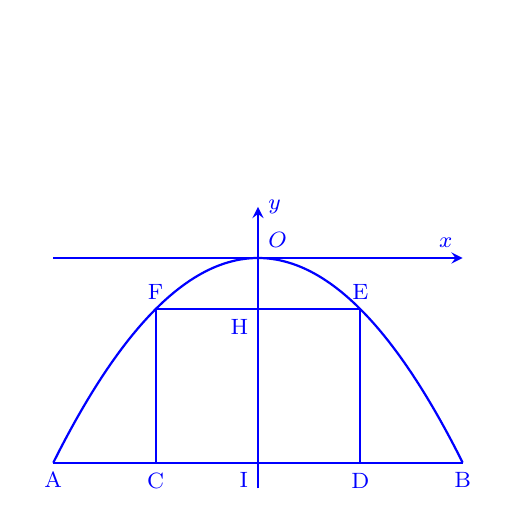
\begin{tikzpicture}[scale=0.65,thick,>=stealth,blue]
				\draw[->] (-4,0) -- (4,0) node [above left] {\footnotesize $x$};
				\draw[->] (0,-4.5) -- (0,1) node [right] {\footnotesize $y$};
				\draw[dashed,thin](2,-1)node[above]{\footnotesize E};
				\draw[dashed,thin](0,-1)node[below left]{\footnotesize H};
				\draw[dashed,thin](0,-4)node[below left]{\footnotesize I};
				\draw[dashed,thin](-2,-1)node[above]{\footnotesize F};
				\draw[dashed,thin](-4,-4)node[below]{\footnotesize A};
				\draw[dashed,thin](4,-4)node[below]{\footnotesize B};
				\draw[thick](2,-1)--(-2,-1)--(-2,-4)node[below]{\footnotesize C}--(2,-4)node[below]{\footnotesize D}--(2,-1);
				\draw[thick](-4,-4)--(4,-4);
				\draw (0,0) node[above right] {\footnotesize $O$};
				\clip (-4.5,-4.5) rectangle (4.5,4.5);
				\draw[smooth,samples=100,domain=-4:4] plot(\x,{-0.25*(\x)^2});
			\end{tikzpicture}
		}
	}
\end{vd}\dongcham{14}

\begin{vd}%[0D2T3]
	\immini{Cổng vào miền Tây (Gateway Arch) ở thành phố St. Louis, nước Mỹ, có hình dạng là một phần của parabol như hình vẽ. Khoảng cách giữa 2 chân cổng $AB=160\,\mathrm{m}$. Trên thành cổng, tại vị trí có độ cao $45\,\mathrm{m}$ so với mặt đất (tại điểm $M$), người ta thả một sợi dây chạm đất (dây căng thẳng theo phương vuông góc với đất). Vị trí chạm đất của đầu sợi dây này cách chân cổng $A$ một đoạn $10\,\mathrm{m}$. Hãy tính khoảng cách từ mặt đất đến điểm cao nhất của cổng.
	}
	{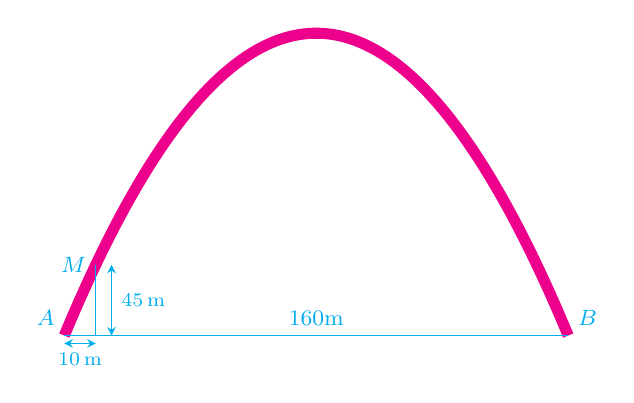
\begin{tikzpicture}[scale=0.2,>=stealth,x=2mm,y=1mm]
			\draw[line width=4pt,magenta,smooth,samples=100,domain=0:160,/pgf/fpu,/pgf/fpu/output format=fixed] plot(\x,{-0.03*(\x)^2+4.8*(\x)});
			\draw[cyan] (0,0) node[above left] {\footnotesize $A$} -- (80,0)node[above] {\footnotesize $160$m}--(160,0) node[above right]{\footnotesize $B$} (10,45) node[left]{\footnotesize $M$};
			\draw[cyan](10,0)--(10,45);
			\draw[<->,thin,cyan](15,0)--(15,45) node[midway,right]{\scriptsize $45\,\mathrm{m}$};
			\draw[<->,thin,cyan] (0,-5)--(10,-5) node[midway,below]{\scriptsize $10\,\mathrm{m}$};
			\usepgflibrary{fpu}
		\end{tikzpicture}
	}
	\loigiai{
		\immini{Đặt hệ trục toạ độ với $Axy$ như hình vẽ.\\
			Xét parabol $(P):\,y=ax^2+bx+c$.\\
			$M\in(P)\Leftrightarrow100a+10b+c=45$\\
			$A\in(P)\Leftrightarrow c=0$. $B\in(P)\Leftrightarrow160^2a+160b+c=0$.\\
			Giải hệ được $y=-0,03x^2+4,8x$.\\
			$\Rightarrow$ Chiều cao cổng là $y(80)=192\,\mathrm{m}$.
		}
		{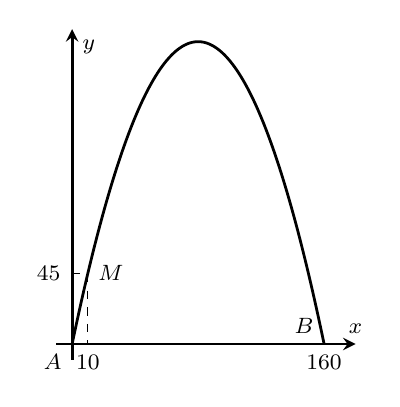
\begin{tikzpicture}[scale=0.2,line width=1pt,>=stealth,x=1mm,y=1mm]
				\draw (0,0) node[below left] {\footnotesize $A$} (10,45) node[right]{\footnotesize $M$} (160,0) node[above left]{\footnotesize $B$};
				\draw[->] (-10,0) -- (180,0) node [above] {\footnotesize$x$};
				\draw[->] (0,-10) -- (0,200) node [below right] {\footnotesize$y$};
				\foreach \x/\xtext in {10/10,160/160}
				\draw[shift={(\x,0)}] (0pt,2pt)--(0pt,-2pt) node[below] {\footnotesize $\xtext$};
				\foreach \y/\ytext in {45/45}
				\draw[shift={(0,\y)}] (2pt,0pt)--(-2pt,0pt) node[left] {\footnotesize $\ytext$};
				\draw[dashed,thin] (0,45)--(10,45)--(10,0);
				\usepgflibrary{fpu}
				\draw[smooth,samples=100,domain=0:160,/pgf/fpu,/pgf/fpu/output format=fixed] plot(\x,{-0.03*(\x)^2+4.8*(\x)});
			\end{tikzpicture}
		}
	}
\end{vd}\dongcham{13}

\begin{vd}%[0D2T3-5]
	Khi quả bóng được đá lên, nó sẽ đạt độ cao nào đó rồi rơi xuống đất. Biết rằng quỹ đạo của quả bóng là một cung parabol trong mặt phẳng với hệ tọa độ $Oth$, trong đó $t$ là thời gian (tính bằng giây), kể từ khi quả bóng được đá lên; $h$ là độ cao (tính bằng mét) của quả bóng. Giả thiết rằng quả bóng được đá lên từ độ cao $1{,}2$ m. Sau đó $1$ giây, nó đạt độ cao $8{,}5$ m và $2$ giây sau khi đá lên, nó ở độ cao $6$ m. Hãy tìm hàm số bậc hai biểu thị độ cao $h$ theo thời gian $t$ và có phần đồ thị trùng với quỹ đạo của quả bóng trong tình huống trên.
	\loigiai
	{
		Gọi $h=at^2+bt+c$ ($a\neq 0$).\\
		Chọn mốc thời gian $t=0$ tại thời điểm quả bóng được đá lên từ độ cao $1{,}2$ m, suy ra $c=1{,}2$. Do đó biểu thức của $h$ có dạng $h=at^2+bt+1{,}2$ ($a\neq 0$).\\
		Tại thời điểm $t=1$ giây nó đạt độ cao $8{,}5$ m nên ta có $a+b=7{,}3$.\\
		Tại thời điểm $t=2$ giây nó đạt độ cao $6$ m nên ta có $4a+2b=4{,}8$.\\
		Như vậy ta có
		\begin{eqnarray*}
			\left\{\begin{aligned}&a+b=7{,}3 \\&4a+2b=4{,}8\end{aligned}\right. \Leftrightarrow \left\{\begin{aligned}&a=-4{,}9 \\&b=12{,}2.  \end{aligned}\right.
		\end{eqnarray*}
		Vậy $h=-4{,}9t^2 + 12{,}2t + 1{,}2$.
	}
\end{vd}\dongcham{8} 

\begin{vd}%[0D2T3-5]
	Chiếc cầu dây văng một nhịp được thiết kế hai bên thành cầu có dạng parabol và được cố định bằng các dây cáp song song.
	\begin{center}
		\begin{tikzpicture}[scale=0.3, font=\footnotesize, line join=round, line cap=round, >=stealth]
			\tikzset{thanh-cau/.pic={
					\draw[scale=0.3,smooth, samples=100, domain=-15:15] plot (\x,{(7/375)*(\x)^2+0.8});
					\foreach \i in {-1.5,-3,-4.5,-6,-7.5,-9,-10.5,-12,-13.5,-15,0,1.5,3,4.5,6,7.5,9,10.5,12,13.5,15} \draw[scale=0.3] (\i,0)--(\i,{(4.2/225)*(\i)^2+0.8});
					\draw[scale=0.3] (-15,0)--(15,0);
			}}
			\path (0,0)pic{thanh-cau};
			\draw [color=gray,fill=cyan!40] (-15,0)--(15,0)--(13,-2)--(-17,-2)--cycle;
			\path (-2,-2)pic{thanh-cau};
			\draw (0,-3.3) node{Hình vẽ cầu dây văng};
			
		\end{tikzpicture}\\
		\vspace{1 cm}
		\begin{tikzpicture}[scale=0.3, font=\footnotesize, line join=round, line cap=round, >=stealth]
			\tikzset{thanh-cau/.pic={
					\draw[scale=0.3,smooth, samples=100, domain=-15:15] plot (\x,{(7/375)*(\x)^2+0.8});
					\foreach \i in {-1.5,-3,-4.5,-6,-7.5,-9,-10.5,-12,-13.5,-15,0,1.5,3,4.5,6,7.5,9,10.5,12,13.5,15} \draw[scale=0.3] (\i,0)--(\i,{(4.2/225)*(\i)^2+0.8});
					\draw[scale=0.3] (-15,0)--(15,0);
			}}
			\path (0,0)pic{thanh-cau};
			\draw[blue,<->] (-15,-0.5)--(15,-0.5);
			\draw[blue,<->] (15.5,0)--(15.5,5);
			\draw[blue,<->] (-15.5,0)--(-15.5,5);
			\draw (15.5,2.5) node[right]{$5$ m};
			\draw (-15.5,2.5) node[left]{$5$ m};
			\draw (0,-0.5) node[below]{$30$ m};
			\draw[<-] (0,0.4)--(2,2) node[above]{$0{,}8$ m};
			\draw (0,-3) node{Hình chiếu đứng của cầu dây văng};
			
		\end{tikzpicture}
	\end{center}
	Dựa vào bản vẽ ở hình bên, hãy tính chiều dài tổng cộng của các dây cáp dọc ở hai mặt bên. Biết
	\begin{itemize}
		\item[] Dây dài nhất là $5$ m, dây ngắn nhất là $0{,}8$ m, khoảng cách giữa các dây bằng nhau.
		\item[] Nhịp cầu dài $30$ m.
		\item[] Cần tính thêm $5$\% chiều dài mỗi sợi dây cáp để neo cố định.
	\end{itemize}
		\loigiai{
		Chọn hệ trục tọa độ sao cho đầu mút $A$ của dây ngắn nhất thuộc trục tung và thanh ngang mặt cầu thuộc trục hoành. Gọi $B$ là điểm đầu mút bên phải (khi nhìn thẳng vào mặt bên của thành cầu) của dây cáp dài nhất thì với các giả thiết:
		\begin{itemize}
			\item Dây dài nhất là $5$ m, dây ngắn nhất là $0{,}8$ m. Khoảng cách giữa các dây bằng nhau.
			\item Nhịp cầu dài $30$ m.
		\end{itemize}
		Ngoài ra, từ bản vẽ ta thấy có tất cả $21$ dây cáp dọc. Suy ra $A(0;0{,}8)$, $B(15;5)$.\\
		Do parabol nhận trục tung là trục đối xứng nên hàm số có công thức $y=f(x)=ax^2+c$.\\
		Ta tìm được $a=\dfrac{4{,}2}{225}$ và $c=0{,}8$. Như vậy $y=\dfrac{4{,}2}{225}x^2+0{,}8$.
		\begin{center}
			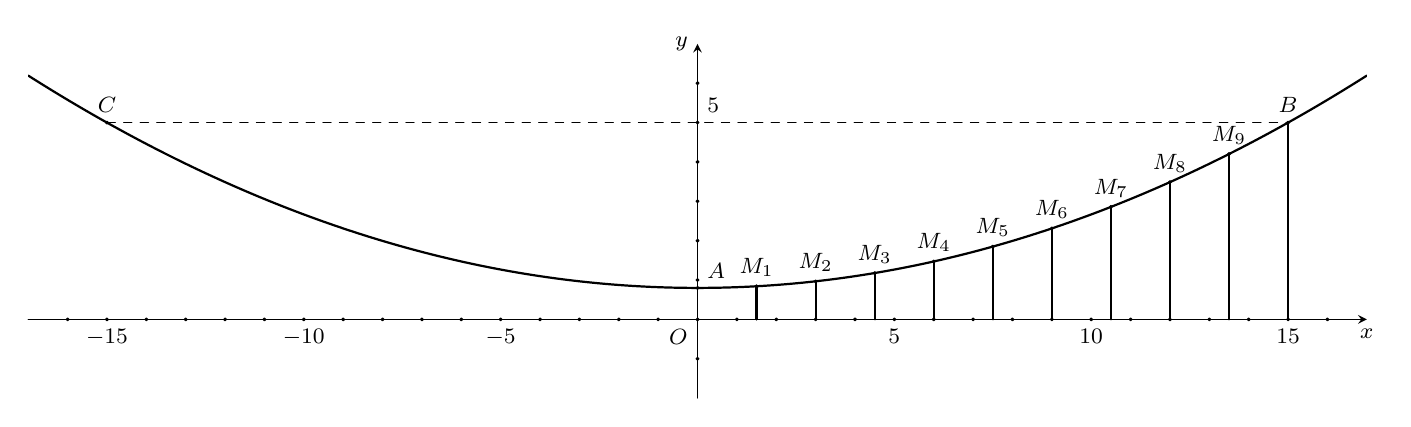
\begin{tikzpicture}[scale=0.5, font=\footnotesize, line join=round, line cap=round, >=stealth]
				\draw [->] (-17,0)--(17,0) node[below]{$x$};
				\draw [->] (0,-2)--(0,7) node[left]{$y$};
				\draw[fill=black] (0,0) circle(1pt) node[below left]{$O$};
				\clip (-17,-2) rectangle (17,7);
				\draw[thick,smooth, samples=300, domain=-17:17] plot (\x,{(7/375)*(\x)^2+0.8});
				\foreach \i in {-15,-10,-5,5,10,15} \draw[fill=black] (\i,0) circle(1pt) node[below]{$\i$};
				\foreach \j in {5} \draw[fill=black] (0,\j) circle(1pt) node[above right]{$\j$};
				\foreach \i in {1.5,3,4.5,6,7.5,9,10.5,12,13.5} \draw [thick](\i,0)--(\i,{(4.2/225)*(\i)^2+0.8});
				\foreach \i/\j in {1.5/1,3/2,4.5/3,6/4,7.5/5,9/6,10.5/7,12/8,13.5/9} \draw [fill=black](\i,{(4.2/225)*(\i)^2+0.8}) circle(1pt) node[above]{$M_\j$};
				\draw[fill=black] (0,0.8) circle(1pt) node[above right]{$A$};
				\draw[fill=black] (15,5) circle(1pt) node[above]{$B$};
				\draw[fill=black] (-15,5) circle(1pt) node[above]{$C$};
				\draw [dashed] (-15,5)--(15,5);
				\draw[thick] (15,0)--(15,5);
				\foreach \i in {-16,-14,-13,-12,-11,-9,-8,-7,-6,-4,-3,-2,-1,1,2,3,4,6,7,8,9,11,12,13,14,16} \draw[fill=black] (\i,0) circle(1pt);
				\foreach \j in {-1,1,2,3,4,6} \draw[fill=black] (0,\j) circle(1pt);
				
			\end{tikzpicture}
		\end{center}
		Chiều dài mỗi dây cáp dọc về mặt lý thuyết là tung độ điểm ứng với đầu mút trên cao của dây cáp, ví dụ dây cáp có đầu mút $A$ có chiều dài bằng tung độ điểm $A$.\\
		Do tính đối xứng, ta có thể xét chiều dài các dây cáp bên phải rồi nhân hai thay vì tính chiều dài tất cả các dây cáp. Riêng dây cáp tại $A$ chỉ tính một lần. Và các dây cáp cách đều nhau nên chiều dài $21$ dây cáp cho một mặt là
		\allowdisplaybreaks
		\begin{eqnarray*}
			L&=& f(0)+2[f(1{,}5)+f(3)+f(4{,}5)+f(6)+f(7{,}5)+f(9)+f(10{,}5)+f(12)+f(13{,}5)+f(15)]\\
			&=& 0{,}8+2\cdot (0{,}842+0{,}968+1{,}178+1{,}472+1{,}850+2{,}312+2{,}858+3{,}488+4{,}202+5)\\
			&=& 49{,}14 \text{ (m).}
		\end{eqnarray*}
		Do cần tính thêm $5$\% chiều dài mỗi sợi dây cáp neo cố định và cần $2$ mặt thành cầu nên chiều dài cáp cần sử dụng cho hai mặt là $2\cdot 49{,}14\cdot 105$\% $=103{,}194$ (m).\\
		Vậy chiều dài cáp cần sử dụng là khoảng $103{,}2$ m.
	}
\end{vd}\dongcham{10}

